%%%%%%%%%%%%%%%%%%%%%%%%%%%%%%%%%%%%
% présenter le framework dans sa vision d'ensemble comme dans WOLFHPC
% faire un joli schéma sous inkscape
% éléments à représenter et expliquer :
%	- MSL language
%	- generic component assembly
%	- MSC compiler
%	- final component assembly
%%%%%%%%%%%%%%%%%%%%%%%%%%%%%%%%%%%%

%----------------------------------------
\subsection{Background on component models}
%----------------------------------------
Component-based software engineering (CBSE) is a domain of software engineering~\cite{Szyperski:2002:CSB:515228} which promotes code
re-use, separations of concerns, and thus maintainability.
An application is made of a set of component instances.
A component is a black box that implements an independent functionality of the application, and which interacts with its environment only through well defined interfaces: its ports.
A port can, for example, specify services provided or required by the component.
With respect to high performance computing, some works have also shown
that component models can achieve the needed level of performance, and
scalability while also helping in application portability~\cite{Bernholdt01052006, bigot:inria-00388508, UCHPC2015}

Many component models exist, each of them with its own specificities.
Well known component models include, for example, the CORBA Component Model (CCM)~\cite{corba:omg06}, and the Grid Component Model (GCM)~\cite{Baude} for distributed computing, while the Common Component Architecture (CCA)~\cite{Bernholdt01052006}, and Low Level Components (\llc)~\cite{l2c} are HPC-oriented.
This work makes use of \llc for the experiments.

\llc~\cite{l2c} is a minimalist \texttt{C++} based HPC-oriented component model
where a component extends the concept of class.
The services offered by the components are specified trough $provide$ ports,
those used either by $use$ ports for a single service instance,
or $use-multiple$ ports for multiple service instances.
Services are specified as \texttt{C++} interfaces.
\llc also offers $MPI$ ports that enable components to share MPI communicators.
Components can also have attribute ports to be configured.
%
As illustrated in Figures~\ref{fig:ports}, a $provide$ port is
represented by a white circle, a $use$
port with a black circle, a $use-multiple$ port by a black circle with
a white $m$ in it. MPI port are
connected with a black rectangle.
A \llc-based application is a static \emph{assembly} of components instances and connections between their ports.
Such an assembly is described in LAD, an XML dialect.

\begin{figure}[t]
\begin{center}
\subfloat[][\label{fig:2comp}]{
\begin{tikzpicture}[shorten >=1pt, node distance=2cm, on grid, auto]
   \node[component] (C) at (0,0) {$c_0$};
   \node[provide] (p) at (-1.5,0) {};
   \node[use] (u) at (1.5,0) {};
   \node[provide,right=1.5cm of u] (p1) {};
   \node[component,right=1.5cm of p1] (C1) {$c_1$};
   \node[use,right=1.5cm of C1] (um) {$m$};
 
  \path[-]
    (p) edge node {$p$} (C)
    (C.east) edge node {$u$} (u)
    (C1)  edge node {$v$} (um)
    (p1) edge node {$q$} (C1);
\end{tikzpicture}
}
\\
\subfloat[][\label{fig:ass}]{
\begin{tikzpicture}[shorten >=1pt, node distance=2cm, on grid, auto]
   \node[component] (C) at (0,0) {$c_0$};
   \node[provide] (p) at (-1.5,0) {};
   \node[use] (u) at (1.5,0) {};
   \node[provide,right=0.15 of u] (p2) {};
   \node[component,right=1.5 of p2] (C1) {$c_1$};
   \node[use,right=1.5 of C1] (um) {$m$};
 
  \path[-]
    (p) edge node {$p$} (C)
    (C) edge node {$u$} (u)
    (C1)  edge node {$v$} (um)
    (p2) edge node {$q$} (C1);
\end{tikzpicture}
}
\\
\subfloat[][\label{fig:mpi}]{
\begin{tikzpicture}[shorten >=1pt, node distance=2cm, on grid, auto]
   \node[component] (C) at (0,0) {$c_2$};
   \node[provide] (p) at (-1.5,0) {};
   \node[mpi] (u) at (1.5,0) {};
   \node[component,right=1.5 of u] (C1) {$c_3$};
 
  \path[-]
    (p) edge node {} (C)
    (C) edge node {} (u)
    (u) edge node {} (C1);
\end{tikzpicture}
}
\caption{Example of components and their ports representation. a) Component $c_0$ has a provide port ($p$) and a use port ($u$); Component $c_1$ has also a provide port ($q$) but also a use multiple port ($v$). b) A use port is connected to a (compatible) provide port. c) Component $c_2$ and $c_3$ shares an MPI communicator.}
\label{fig:ports}
\end{center}
\end{figure}

%----------------------------------------
\subsection{Multi-Stencil Framework overview}
%----------------------------------------

\begin{figure}[t]
\begin{center}
  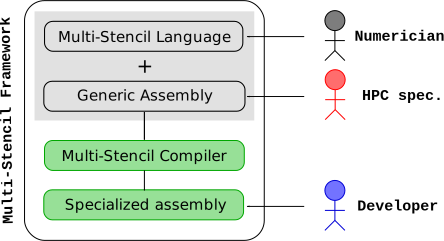
\includegraphics[width=.6\textwidth]{./images/msf.pdf}
  \caption{The Multi-Stencil Framework (MSF) composed of the Multi-Stencil Language (MSL), the Generic Assembly (GA), the Multi-Stencil Compiler (MSC) and which produces a specialized assembly of components.}
  \label{fig:msf}
\end{center}
\end{figure}